% !TEX root = ../thesis-example.tex
\chapter{Concepts}
\label{sec:concepts}

In this Chapter different ways to evaluate TeSSLa specifications are given and their equivalence is shown.
To do so in Section~\ref{sec:concepts:defs} building blocks for evaluation approaches are defined, which are then used in later Sections to define behaviour of them and show their equivalence.

\section{Definitions}
\label{sec:concepts:defs}

While the TeSSLa specification itself defines a set of semantics, for this Thesis we will slightly alter some of it and add some new definitions based on them.
This is necessary to reason about the specifics how the evaluation engine is built (Note that TeSSLa doesn't define an operational semantic, therefore we will define our own) and how it behaves.

\subsection{Events}
\label{sec:concepts:defs:events}

Events are the atomic unit of information that all computations are based on.
There are three Types of Events: input, output and internal Events.

The Set of all Events is denoted as \(E\).
Each event carries a value, which can be \emph{nothing} or a value of a Type (types are formally defined in the TeSSLa speicification but aren't important for this thesis), a timestamp and the stream it's perceived on (e.g.\ a function call of a specific function or the name of an output stream).

The value of an event can be queried with the function \(\upsilon\), its timestamp with \(\pi\) and its Stream with \(\varsigma\).

\(E_i \subset E\) is the Set of all input events, their Stream corresponds to a specific trace.
\(E_o \subset E\) is the Set of all output events, their Stream is specified by an output name of the TeSSLa specification.
\(E_n \subset E\) is the Set of all internal events.
Internal events are mostly an implementation detail, which denote steps of computation inside the runtime.
The Stream of internal events is implicitly given by the node that produces the stream of the Event.
Note that \(E_i, E_o, E_n\) are pairwise disjoint and \(E_i \cup E_o \cup E_n = E\).

\subsection{Streams}
\label{sec:concepts:defs:streams}

Stream are a collection of Events with some added characteristics.
While Events are the atomic unit of information, Streams represent the sequence of related Events over time.

There are two kind of Streams: Signals, which carry values at all times, and EventStreams, which only hold values at specific times.
EventStreams can be described by a sequence of Events.
Signals can be described by a sequence of changes, where a change notes that the value of a Signal changed at a specific timestamp.
The only difference between a Signal and an EventStreams is that Signals always have a value while an EventStream may return \(\bot\), which denotes, that no event happened at that time.
Because the similarity of Signals and EventStreams in the following we will mainly reason about EventStreams, but most things can also be applied to Signals.

Formally a Stream \(\sigma\) can be represented as a Sequence of Events \(\langle e_1, \dots e_n\rangle\) where \(\pi(e_i) < \pi(e_{i+1}) \forall i < n \in \mathbb{N}\).
The Set of all Streams \(\Sigma\) is defined as all possible finite sequences of Events \(\Sigma = \{\sigma | \sigma \in E^* \}\).
An input Stream \(\sigma_i\) is a stream consisting only of input Events, the set of all input Streams is \(\Sigma_i = \{\sigma_i | \sigma_i \in E_i^*\}\).
Output and internal Streams are defined analogous.
To get the Event of a Stream \(\sigma\) at a timestamp \(t\) it can be queried like a function: \(\sigma(t) = e\) with \(\pi(e) = t \).
When working with Signals, the function will return the latest Event that happened at or before t while an EventStream may return \(\bot\).

Furthermore Streams hold the timestamp to which they have progressed, which can be equal or greater than the timestamp of the last Event happened on them.


\subsection{Functions}
\label{sec:concepts:defs:functions}

A TeSSLa specification consists of functions.
Functions generate new Streams by applying an operation on other Streams.
TeSSLa itself defines a syntax to write a specification, a set of types and a standard library of functions, but an implementation is free to choose the functions it supports.

An example function is \(add(S_D,S_D) \rightarrow S_D\): It takes two Signals, which have to hold values of some numerical type, and produces a signal which holds values of the same type.
The produced stream can either be assigned to a named identifier (think: a variable) or directly be given to another function (function composition).

Functions can be divided into three categories: pure, unpure and timing.
Pure Functions, also called stateless, are evaluated only on the values their inputs have at the timestamp they are evaluated, therefore they don't have to \emph{remember} anything about earlier events.
Unpure, or stateful, Functions are evaluatet over the whole input stream, meaning they can look at all Events that happened on its inputs before the time of evaluation and also at all it's previous output events.
E.g.\ a Function \emph{eventCount} has to \emph{remember} how many events already happened on it's input stream and increment that counter on every new event.
Timing Functions are evaluated not only on the value of Events but also on their timestamp and can also manipulate it:
While non timing functions will consume events at a specific timestamp and emit an event with that timestamp, timing functions can emit Events with a different timestamp.

Timing Functions complicate the reasoning about schedules and causality and therefore aren't included in Section~\ref{sec:concepts:behaviour_without_timing}.
In Section~\ref{sec:concepts:behaviour_with_timing} the conclusions of earlier sections will be extended to include timing functions.


\subsection{Nodes}
\label{sec:concepts:defs:nodes}

Nodes are the atomic unit of computation for the evaluation of a TeSSLa specification.
A Node implements a single Function, e.g.:\ there is an \emph{AddNode} which takes two input Signals and produces a new Signal.
Therefore a Node is the concrete implementation of a function in a runtime for TeSSLa specifications.
Each Node has a set of inputs, which are either input or internal Streams, and one output, which is either an internal or an output Stream.


Nodes use a FIFO queue, provided by the Erlang plattform, to process new received Events in multiple steps:

\begin{enumerate}
  \item Add the new Event to the inputs
  \item Check if a new output Event can be produced (see Section~\ref{sec:concepts:defs:nodes:processable})
  \item If so, compute all timestamps, where new Events might be computed and
    \begin{enumerate}
      \item Compute the Events, add them to the History as new outputs
      \item Distribute the updated output to all successors
    \end{enumerate}
  \item Else wait for another input
\end{enumerate}

\subsubsection{Determination of processable Events}
\label{sec:concepts:defs:nodes:processable}

Based on the asynchronous nature of Nodes, Events from different Streams can be received out of order.
E.g.\ if a Node C is a child of Node A and B, it can receive Events from Node A at timestamps \(t_1, t_2, t_3, t_4\)
before receiving an event with timestamp \(t_1\) from Node B.
Therefore a Node can not compute it's output upto a timestamp unless it has informations from all predecessors that they did progress to that timestamp.
When Node C receives the first four Events from Node A, it will only add them to it's inputs but won't compute an output.
When it finally receives the first Event from Node B it can compute all Events upto \(t_1\).
To do so it will compute \emph{change timestamps}: The union of all timestamps where an Event occured on any input between the timestamp of the last generated output and the minimal progress of all inputs.

To see why this is necessary lets assume that Node C will receive a new Event from Node B with timestamp \(t_4\):
All inputs have progressed to \(t_4\), but on the stream from Node A there are changes between \(t_1\) (where the last output was generated) and \(t_4\),
therefore the \emph{change timestamps} are \(t_2, t_3, t_4\) and the Node will have to compute it's output based on the values of the streams at that timestamps.

\subsection{TeSSLa Evaluation Engine}
\label{sec:concepts:def:model}

Because Functions in TeSSLa specifications itself depend on other Functions, and these dependencies have to be circle free,
the specification can be represented as a DAG@.
This DAG can be directly translated into an evaluation Engine for that specification: The Nodes of the DAGs are Nodes representing the functions and the Edges are the input and output Streams between the Nodes.

\begin{definition}[name=Equality of evaluation Engines]\label{def:equality_eval_engine}
  Two evaluation Engines are called equal, if they produce the same Relationship between inputs and outputs for all possible inputs.
\end{definition}

\begin{definition}[name=Equality of evaluation Engines]\label{def:equality_eval_engine_specific}
  Two evaluation Engines are called equal for an input, if they produce the same output for that input.
\end{definition}

\begin{definition}[name = Enabledness of Nodes]\label{def:node_enabled}
  A Node in the DAG is called \emph{enabled} when it has at least one Event buffered on all of it's inputs, meaning it is able to perform a computation and produce a new output.
  In the context of a Run enabledness means, that a Transition can be taken which represents the computation of the enabled Node.
\end{definition}

\begin{definition}[name = Equality of evaluation Engines]\label{def:node_independent}
  A Node in the DAG is called \emph{independent} of another Node, if it is no descendant of that Node.
\end{definition}

\begin{lemma}[name = Duration of Enabledness]\label{lemma:enabled_till_scheduled}
  A Node which is enabled stays enabled until it is scheduled
\end{lemma}

\begin{proof}
TODO
\end{proof}


To evaluate a specification over Traces, the Evaluation Engine has process the Events that were traced.
To do so the Nodes have to run their computations until no more Events are present (or the specification found an error in the trace).
This leads to the question in which order Nodes should be scheduled to perform their computation.
While some schedules are simply not rational (think of unfairness and causality) there are many different schedules that are feasible.
It has to be prooven that a chosen schedule produces the correct conclusions for a specification, else the Evaluation Engine is not valid.

In this Thesis it is shown that multiple schedules will lead to the same conclusions and therefore an implementation of an Evaluation Engine is free to choose between them.

\subsection{State}
\label{sec:concepts:def:state}

All TeSSLa evaluation Engines have to hold a State, which encodes information necessary to continue the evaluation.
The State of a whole Evaluation Engine is made up of the States of it's Nodes.

Each Node has a State which holds the History of its input Streams and its output Stream.
One part of the State of every Node is the History of a Node, which holds all Events received from it's parents, called it's inputs, and all produced Events of the Node, called it's output.

To distinguish between the two types of States, we will call the State of the whole Engine the \emph{global State} and the State of a Node the \emph{Node State}.

Formally the State of a Node is a tuple of the inputs (a Set of internal and input Streams) and the output (an internal or an output Stream).
The Set of all valid States of a Node is \(N = {(\Sigma_i \cup \Sigma_n)}^*\times(\Sigma_n \cup \Sigma_o)\).
Based on this, the Set of all valid States is \(S = N^*\).
A global State can be queried like \(S_1(i) = n_i\) to yield the State of the Node at that position.

Everytime a Node is scheduled it changes it State by:

\begin{itemize}
  \item Updating it's inputs (Adding a new Event to the Input Streams)
  \item Generating a new Event if possible and add it to it's outputs
\end{itemize}

\subsection{Transitions}
\label{sec:concepts:def:transitions}

A Transition describes what happens when the evaluation Engine switches State by performing a Step:
The consumption of one Event from each input of a Node and the optional generation of one or more new output Events of that Node.
To look at it in another way: A Transition is the computation of a Node, therefore when we say `Node A is scheduled' we mean that a Transition is taken which models the computation of that Node.

Formally Transitions are a Relation between two Sets of Events.
E.g.\ the Transition \(\tau = (\{e_1,e_2\}, \{e_3\})\) specifies that two Events were consumed by a Node (thereby adding them to its inputs) and one Event was produced based on them (which is added to the output).
The Set of all Transitions is
\[
  T = \{(e, e') | e \subseteq (E_i \cup E_n),e \neq \emptyset, e' \subseteq (E_n \cup E_o), \forall e_i, e_j \in e': \varsigma(e_i) = \varsigma(e_j)\}
\]
where the Node which caused the Transition is the one creating the Stream \(\varsigma(e_i)\).

The empty Transition, meaning no input was consumed and no output produced, is labeled with \(\lambda\).
Note that all Transitions, except the empty one, have to consume at least one Event (therefore no Events can be created from nowhere) and that it's possible that no Event was produced based on the consumed Events (think of a \emph{FilterNode}).
Furthermore it's theoretically possible to create multiple Events in one Transition.
This makes only sense in the context of Timing Nodes, because else the generated Events would have the same timestamp, which is forbidden by the definition of Streams.
With Timing Nodes one could for example implement an \emph{EchoNode}, which duplicates an input after a specified amount of Time.

\begin{definition}[name = Independence of Transitions]\label{def:independence_transitions}
  A Transition is called independent of another, if the Node of which it represents the computation, is independent of the Node of the other Transition.
\end{definition}


\subsection{Run}
\label{sec:concepts:def:run}

A Run of an Evaluation Engine is a Sequence of Transitions and States.
The first element of the sequence is the empty Transition and the initial State of the evaluation Engine.
It is a representation of the steps the Engine takes to evaluate a specification over input Streams.
The Run \(\langle (\lambda, s_0), (\tau_1, s_1) \rangle\) means, that the Engine was in it's initial State, took the transition \(\tau_1\) and thereby reached the state \(s_1\).

\begin{definition}[name = Equality of Runs]\label{def:equal_runs}
  Two Runs are called equal if they have the same State at their last position.
\end{definition}

Because the State can be built from the Transitions that were taken, equality can also be defined over Transitions.

\begin{lemma}[name = Equality of Runs over Transitions]\label{lemma:equal_runs_with_transitions}
  If the Set of Transitions of two Runs are equal, the Runs are equal.
\end{lemma}

\begin{proof}
  Let \(R_1, R_2\) be the Runs of two Engines with the same Set of Transitions \(T'\).
  Let \(S_1\) be the final State of the Run \(R_1\) and \(S_2\) of \(R_2\).
  If the two global States weren't equal, there would have to be at least one \(i\) with \(S_1(i) \neq S_2(i)\), meaning the same Node has to have a different State in both Engines.
  Let \(n_1, n_2\) be the States of one such Node in both Engines.
  If the two States are different, one of them has to contain at least one Event on an input or output that isn't on the same Stream in the other State.
  Let that Event be \(e_d\).
  To be added to the State, there has to be a Transition \(\tau = (e, e')\) with \(e_d \in e \lor e_d \in e'\).
  This Transition has to be in \(T'\), which means it was taken by both Engines, therefore \(e_d\) is in the History of the Node in both Runs.
\end{proof}

\begin{definition}[name = Distance of Runs]\label{def:runs_distance}
  The Distance \(\delta\) of a Run \(R_1\) to a Run \(R_2\) is a pair \(\delta(R_1,R_2) = (x,y)\), where \(x\) is the index before the first position where the two Runs differ and y is the number of Steps between the index of the first difference and the position where \(R_2\) takes the Transition that \(R_1\) took after step \(x\).
  The Distance of Runs is compared element-wise: \((x,y) < (x',y') \leftrightarrow ((x > x') \lor (x = x' \land y < y))\).
\end{definition}

\begin{exmp}
  Let
  \[R_1 = \langle (\lambda, S_0), (\tau_1,S_1), (\tau_2,S_2), (\tau_3,S_3), (\tau_4,S_4), (\tau_5,S_5), (\tau_6,S_6) \rangle\]
  \[R_2 = \langle (\lambda, S_0), (\tau_1,S_1), (\tau_2,S_2), (\tau_5,S_3'), (\tau_4,S_4'), (\tau_6,S_5'), (\tau_3,S_6') \rangle\]
  \[R_3 = \langle (\lambda, S_0), (\tau_1,S_1), (\tau_2,S_2), (\tau_3,S_3), (\tau_5,S_4''), (\tau_4,S_5''), (\tau_6,S_6'') \rangle\]

  Than is
  \[\delta_{1,2} = \delta(R_1,R_2) = (3,3),\ \delta_{1,3} = \delta(R_1,R_3) = (4,1)\]
  \[\delta_{2,1} = \delta(R_2,R_1) = (3,2),\ \delta_{2,3} = \delta(R_2,R_3) = (3,1)\]
  \[\delta_{3,1} = \delta(R_3,R_1) = (4,1),\ \delta_{3,2} = \delta(R_3,R_2) = (3,2)\]

  And \(\delta_{1,3} < \delta_{2,3} < \delta_{2,1} < \delta_{2,1}\).


\end{exmp}

\begin{lemma}[name = Influence of independent Nodes]\label{lemma:independence}
  When a Node A is independent of a Node B, than it has no influence on the enabledness of Node A if Node B is scheduled before or after it.
\end{lemma}

\begin{proof}
  As already shown in Lemma~\ref{lemma:enabled_till_scheduled}, if Node A is enabled, it stays enabled until it's scheduled, so the computation of B can't change A from enabled to disabled.
  It remains to show, that the computation of Node B can't change Node A from disabled to enabled.
  A Node becomes enabled when on all of its input at least one new Event is present.
  New Events on an input are added, when a parent Node performs computation.
  Because A is independent of B, no input of A is the output of B.
  Furthermore B is no parent of any predecessor of A, therefore no predecessors input is the output of B.
  Because of that, when B is scheduled, no Event can be added to the input of any of A's predecessors or A itself.
  So if A wasn't enabled earlier because it hasn't a new Event at one input, the computation of B can't lead to adding that Event.
  Therefore it doesn't at which position B is scheduled in regard to the enabledness of A.
\end{proof}

\section{Behaviour of different schedules without timing functions}
\label{sec:concepts:behaviour_without_timing}

For a first step we specify and compare behaviours of different approaches to evaluate TeSSLa specifications without timing Functions.
Without timing Functions, all Nodes work only on values or the presence of Events.
This leads to behaviours that can be easily reason about, as seen in the next sections.

All Systems to evaluate TeSSLa specifications we will look at are based on the described structure in Section~\ref{sec:concepts:def:model}.
While there may be other approaches to evaluation, a DAG based approach seems to fit most naturaly and focusing on one structure makes comparing Systems easier.

Each evaluation Engine will work in steps, where each step is synonymous with an index in the Run of the System.
Therefore at each Step one Node is scheduled to perform it's operation, represented as the Transition in the Run.
The Transition will encode one of the following three Things that can happen:

\begin{itemize}
  \item An input Event can be consumed by a source in the DAG, which generates an internal Event that is propagated to it's children.
  \item An internal Node, which has at least one new input buffered on all of its input queues, can perform
    its computation and generate a new internal Event, which is propagated to the children of that node, which therefore can compute in the next step.
  \item An output node, which has at least one new input buffered on all of its input queues, can produce a new output.
\end{itemize}

Evaluation Engines are free in the way they are scheduling their Nodes, only limited by causality (no Event can be consumed before it's produced).
In the following evaluation Engines are classified by their scheduling approaches.

\subsection{Synchronous Evaluation Engines}
\label{sec:concepts:behaviour_without_timing:synchronous}

The first class of evaluation Engines are synchronous ones.
They are characterized by a specific, fixed schedule.
The scheduling algorithm is as follows: Choose a reversed topological order of the Nodes once and assign numbers to them in that order.
Then always schedule the enabled Node with lowest Number.

Obviously for many DAGs there is no unique reversed topological order, therefore one can be chosen by the evaluation engine.

This schedule ensures that no Node is scheduled which has a successor that can be scheduled, therefore Events are \emph{pushed} through the DAG towards an output Node as fast as possible.

\begin{definition}[name = Equality of evaluation Engines]\label{def:valid_eval_engine}
  An evaluation Engine is called \emph{valid}, if it is equal to a synchronous evaluation Engine.
\end{definition}

% As shown in Section~\ref{sec:concepts:equalitys_without_timing} all synchronous evaluation Engines are equal.
% Therefore to proof that an evaluation Engine is valid for a specification, one has to show, that it is equal to any synchronous one.

\begin{figure}
  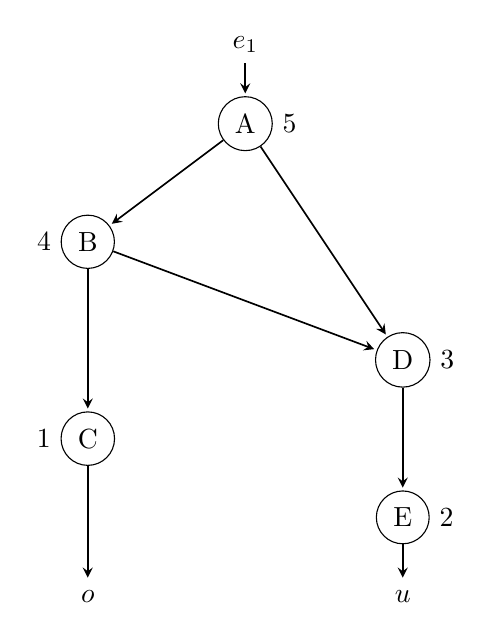
\begin{tikzpicture}
    [pre/.style={<-,shorten <=1pt,>=stealth,semithick}]
    \node (S) at (2,5) {\(e_1\)};
    \node [shape=circle,draw=black] (A) [label=right:5] at (2, 4) {A}
      edge [pre] (S);
    \node [shape=circle,draw=black] (B) [label=left:4] at (0,2.5) {B}
      edge [pre] (A);
    \node [shape=circle,draw=black] (C) [label=left:1] at (0,0) {C}
      edge [pre] (B);
    \node [shape=circle,draw=black] (D) [label=right:3] at (4,1) {D}
      edge [pre] (A)
      edge [pre] (B);
    \node [shape=circle,draw=black] (E) [label=right:2] at (4,-1) {E}
      edge [pre] (D);
    \node (o1) at (0,-2) {\(o\)} edge [pre] (C);
    \node (o2) at (4,-2) {\(u\)} edge [pre] (E);
  \end{tikzpicture}
  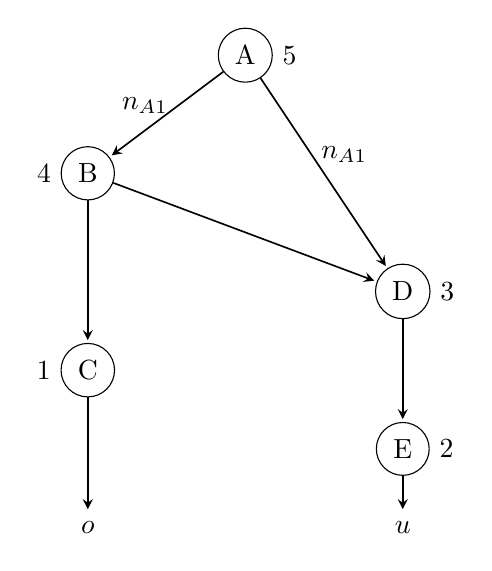
\begin{tikzpicture}
    [pre/.style={<-,shorten <=1pt,>=stealth,semithick}]
    \node [shape=circle,draw=black] (A) [label=right:5] at (2, 4) {A};
    \node [shape=circle,draw=black] (B) [label=left:4] at (0,2.5) {B}
      edge [pre] node[align=left,left,pos=0.6] {\(n_{A1}\)} (A);
    \node [shape=circle,draw=black] (C) [label=left:1] at (0,0) {C}
      edge [pre] (B);
    \node [shape=circle,draw=black] (D) [label=right:3] at (4,1) {D}
      edge [pre] node[align=right,right,pos=0.6] {\(n_{A1}\)} (A)
      edge [pre] (B);
    \node [shape=circle,draw=black] (E) [label=right:2] at (4,-1) {E}
      edge [pre] (D);
    \node (o1) at (0,-2) {\(o\)} edge [pre] (C);
    \node (o2) at (4,-2) {\(u\)} edge [pre] (E);
  \end{tikzpicture}
  \caption{Visualization of a simple asynchronous system with a reversed topological order.}
\label{fig:chap3:sec_sync:visual_dag}
\end{figure}

Figure~\ref{fig:chap3:sec_sync:visual_dag} visualizes a synchronous evaluation Engine.
It shows two DAG representations of an evaluation Engine  where the Nodes A to E are labeled in a reversed topological order and \(o\) and \(u\) represents the output Streams with that name.
The left System is in it's initial State and an input event \(e_1\) is present and can be consumed by the input Node A.
When a Node is chosen to compute by the scheduler, only Node A is enabled, therefore it is scheduled.
The right system is the representation of the next step: Node A has consumed the external event and produced an internal event \(n_{A1}\) which is propagated to all it's children: Node B and D.
In the next step Node B would be scheduled, because it has the lowest number of any node that can compute (actually it's the only node that can compute at all, because D has to wait for the event from B).
After B was scheduled, it would have produced the internal Event \(n_{B1}\) which would then be distributed to Nodes C and D.

The complete Run of the synchronous Engine for one Input is the following, where the States are not further defined:

\begin{align*}
  \langle
    (\lambda,                             S_0),
    ((\{ n_{A1}         \}, \{n_{B1}\}),  S_1),
    ((\{ n_{B1}         \}, \{o_1\}),     S_2),\\
    ((\{ n_{A1}, n_{B1} \}, \{n_{D1}\}),  S_3),
    ((\{ n_{D1}         \}, \{u_1\}),     S_4)
  \rangle
\end{align*}

If there were more than one input Event, at this point Node A would be scheduled again.
It would consume the next input and the following Nodes would be scheduled in the same order as before, extending the Run in an obvious way.

\subsection{Asynchronous evaluation}
\label{sec:concepts:behaviour_without_timing:async}

An asynchronous evaluation Engine one with a fair, but not fixed schedule.

In contrast to the synchronous evaluation Engine it has no fixed schedule, the only requirement is that the schedule is fair.
Therefore predecessors of enabled Nodes can perform multiple computations before their children are scheduled and Events are not \emph{pushed} through the DAG as fast as possible.
\todo{more later}

\section{Equalitys of different schedules without timing functions}
\label{sec:concepts:equalitys_without_timing}

Based on the described behaviours of the approaches we now can proof the equality of different Schedules for the same evaluation Engine for a TeSSLa specification.

\begin{lemma}[name = Equality of Engines for one Input]\label{lemma:eval_equal_if_runs_equal}
  Two evaluation Engines are equal for an input, if their Runs are equal for that input.
\end{lemma}

\begin{proof}
  Since two Runs are equal if they have the same last State, and all Events which were produced are stored in the State, during both Runs the same output Events had to be generated or else their State would differ.
\end{proof}

% Two Runs are assumed to be equal if the State of their last elements are equal:
% Because all generated Events are saved in the State of an Engine, if two Runs have the same State in their last element they did produce the same outputs.


As defined by Definition~\ref{def:valid_eval_engine} any evaluation Engine has to be equal to a synchronous to be valid.

The Equality is shown in two steps: First in Section~\ref{sec:concepts:equalitys_without_timing:synchronous} it is shown, that all possible synchronous Engines for a specification are equal, so there is only one valid Evaluation.
Afterwards in Section~\ref{sec:concepts:equalitys_without_timing:sync_async} it is shown that any asynchronous evaluation Engine is equal to a synchronous one.


\subsection{Equality of synchronous Systems}
\label{sec:concepts:equalitys_without_timing:synchronous}

When given a series of input Events, two synchronous evaluation Engines for a specification with different schedules will have different Runs.
But both will produce all outputs that can be produced after consuming one specific input before the next Input is consumed as reasoned in Section~\ref{sec:concepts:behaviour_without_timing:synchronous}.
Also both Runs will obviously have the same length (both Engines are the same DAG, so they have the same number of Nodes), let that length be \(l\).

To proof the equality of both Engines we have to proof the equality of their Runs.
To show the equality we will show that there is always another Run, which is equal to the second one, that has a smaller Distance from the first one.
If such a closer Run always exist, we will show that the Run with Distance \(l, 0\) to the first Run, which has to be the first Run itself, is also an equal Run to the second Run.

\begin{theorem}[name = Equality of different synchronous evaluation Engines]\label{theorem:equal_sync_eval_engines}
  Two synchronous evaluation Engines for a specification with different schedules are equal.
\end{theorem}
\begin{proof}

% Let \(\vec{e} = (e_1, e_2, \dots, e_x)\) be the input Events both Engines receive.
Let \(R_1, R_2\) be the Runs of the two Engines for a given TeSSLa specification.
Because each TeSSLa specification contains only a finite amount of Functions and works on finite traces, the Runs also have to be finite.

If the two Runs aren't equal, they must have a Distance which is bigger than \((l, 0)\).
Let \([R_2]\) be the Set of all Runs that are equal to \(R_2\).
All of those Runs will also have a Distance from \(R_1\) which is bigger than \((l, 0)\).
Select one Run \(R_2' \in [R_2]\) which has a minimal Distance from \(R_1\).
Let \((d,k) = \delta(R_1, R_2')\).

This means that at Step \(d\) the Run \(R_2'\) has taken a different Transition than Run \(R_1\).
Let the Transitions the Runs have taken be \(\tau_1\) for \(R_1\) and \(\tau_2\) for \(R_2'\).
Run \(R_2'\) will take Transition \(\tau_1\) at step \(d+k\) (as per the definition of the Distance).
Obviously the two Transitions have to be independent of each other, else they couldn't have been taken in different order by the two Runs.

If \(k > 1\) there will be a Transition \(\tau_2' \neq \tau_1\) which is taken by the Run \(R_2'\) at Step \(d+(k-1)\).
While this Transition \(\tau_2'\) must also be taken in the first Run as per Lemma~\ref{lemma:enabled_till_scheduled}, it's not possible, that it was taken before \(\tau_1\), beause than the two runs wouldn't have been the same upto the point where \(\tau_1\) was taken.
Therefore \(\tau_1\) has to be independent of \(\tau_2'\), and because \(\tau_2'\) was scheduled by the second Run before \(\tau_1\) both Transitions are independent of each other.

As of Lemma~\ref{lemma:independence} which one of them is taken first can't change the enabledness of the Node of the second Transition.
Therefore there is a Run \(R_2''\) which is exactly the same to \(R_2'\), except that the Transitions \(\tau_1, \tau_2'\) are scheduled the other way around.
Figure~\ref{fig:chap3:sec_sync:commutativity_scheduling} visualizes how changing the order of the two Transitions can't change the global State of the Engine after both were taken.
Therefore the Runs \(R_2'\) and \(R_2''\) are equal and the Distance to \(R_1\) is \(d, k-1\), which contradicts the initial statement that \(R_1'\) was a Run with a minimal Distance.
This means that there is an equal Run to \(R_2\) which has at most the Distance \((d, 1)\).

If \(k = 1\) the Transition \(\tau_2'\) from the previous case is equal to \(\tau_2\).
Based on the same reasoning there also exist a Run \(R_2''\) which is exactly the same to \(R_2'\) except that the order of \(\tau_2\) and \(\tau_1\) is changed, and which is also equal to \(R_2'\) and to \(R_2\).
This Run has the Distance \((d, 0)\) from \(R_1\).
This obviously doesn't make sense: The first element of the Distance is the last step where both Runs are equal, the second element describes how many Steps afterwards the differing Transition was taken.
But if it was taken right in the Step after the last equal Step, there is no difference at that position, so the Difference of \(R_1\) and \(R_2''\) can be at most \((d+1, x), x \in \mathbb{N}_{>0}\).
This also contradicts our initial Statement that \(R_2'\) was the Run with the smallest Distance from \(R_1\) which is equal to \(R_2\).

Combined we can now say, that there is no lower bound on the Distance of equal Runs of \(R_2\) to \(R_1\), therefore the Run with the Distance \((l, 0)\) also has to be equal to \(R_2\).

\end{proof}


% Let \(N_1\) be the Node scheduled by the first evaluation Engine and \(N_2\) the one scheduled by the second.
% Because \(N_1\) was scheduled by the first evaluation Engine and upto \(i_d\) the two Engines took the same steps it also has to be enabled in the second Engine, and because it wasn't scheduled by it, it has to still be enabled after that step.
% The same holds for \(N_2\) in the first evaluation engine.

% After step \(i_d\) both system might take a finite number of different transitions, but at some point the first System has to schedule Node \(N_2\) and the second system Node \(N_1\), because there are only a finite number of Nodes with a lower number and a Node can only become \emph{not enabled} by performing it's computation.
% Let \(i_{N_2} > i_d\) be the index of the step where the first System schedules the Node \(N_2\).
% Let \(N_b\) be the set of all Nodes which were scheduled between \(i_d\) and \(i_{N_2}\).
% All of theese Nodes have to be independent of \(N_2\), because otherwise they couldn't be scheduled before \(N_2\). %, because they would have had to wait for an Event from \(N_2\).
% On the other hand \(N_2\) has to be independent of all Nodes in \(N_b\) because otherwise it couldn't have been scheduled before them in the second evaluation Engine.

% Now let \(N_c \in N_b\) be the Node that was scheduled at step \(i_{N_2} - 1\) and
% \(r_s = (\langle \tau_{i_{N_2} - 2}, s_{i_{N_2} - 2}\rangle, \langle\tau_{i_{N_2} - 1}, s_{i_{N_2} - 1}\rangle \langle\tau_{i_{N_2}}, s_{i_{N_2}}\rangle)\)
% the infix of the Run of the first Engine, starting two steps before \(N_2\) was scheduled upto the point where it was scheduled.

\begin{figure}
  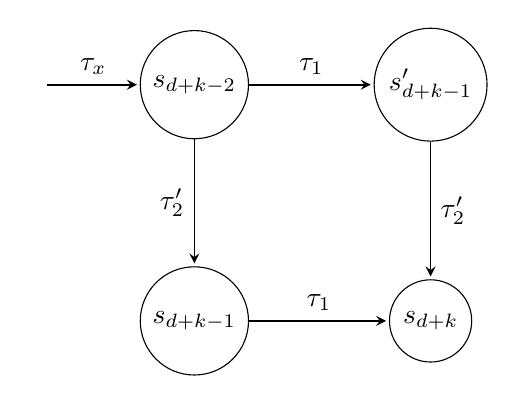
\begin{tikzpicture}
    [pre/.style={<-,shorten <=1pt,>=stealth,semithick}]
    \node (A) at (0,0) {};
    \node [shape=circle,draw=black] (B) at (2, 0) {\(s_{d+k-2}\)}
      edge [pre] node[above] {\(\tau_{x}\)} (A);
    \node [shape=circle,draw=black] (C) at (2, -3) {\(s_{d+k-1}\)}
      edge [pre] node[left] {\(\tau_{2}'\)} (B);
    \node [shape=circle,draw=black] (D) at (5, 0) {\(s_{d+k-1}'\)}
      edge [pre] node[above] {\(\tau_{1}\)} (B);
    \node [shape=circle,draw=black] (E) at (5, -3) {\(s_{d+k}\)}
      edge [pre] node[right] {\(\tau_{2}'\)} (D)
      edge [pre] node[above] {\(\tau_{1}\)} (C);
  \end{tikzpicture}
  \caption{Commutativity Diagramm of Node scheduling}
\label{fig:chap3:sec_sync:commutativity_scheduling}
\end{figure}

% \todo{The praragraph is a bit handwavy, needs more formal definitions}
% Figure~\ref{fig:chap3:sec_sync:commutativity_scheduling} visualizes how changing the order of the Nodes \(N_c, N_2\) has no influence on the global State after both have executed.
% This follows from the fact, that both Nodes are independent of each other as shown before.
% This means that the computation of one of them can't change the State of the other, thereby having absolutely no consequence on the computation of the other.
% If both Nodes have mutual children, that children will receive their inputs in different order, but because the events are  on different Streams it doesn't matter.
% Therefore it doesn't matter which of the both Nodes is scheduled first: the state of the system will be different only at one position, but afterwards they both will have the same State again.
% If one of the Nodes generate an output event, that event will be emitted one step earlier or later, which is also not relevant for the global State.

% To summarize: The order of computation of the Node \(N_2\) and the one scheduled before it doesn't change the State of the Evaluation Engine after both have run.
% Therefore their order can be changed, which generates a new Run which is equal to the old one.

% This reordering can be repeated until \(N_2\) is scheduled right after \(N_1\), because as shown earlier \(N_2\) has to be independent of all Nodes between the two.
% Now \(N_1\) and \(N_2\) also have to be independent, else one of them couldn't have been scheduled before the other.
% Therefore the two can be also reordered without changing the final State.
% After this reordering, both Runs will have a final prefix \(R''\), which length has to be at least one more than \(R'\).

% Now the reordering can be repeated for the next index where the first difference between the runs happen.
% Everytime the reordering for one index finishes the finite, equal prefix will has at least one more position, therefore at one Point both runs are equal, because the Prefix is the run itself.


\subsection{Equality of synchronous and asynchronous schedules}
\label{sec:concepts:equalitys_without_timing:sync_async}

When the Nodes of \(A\) aren't scheduled in reversed topological order, the system can consume Inputs before producing all outputs based on the last consumed Input.
Therefore the reordering of runs has to be performed over wider parts of the run.
% Idea: each step is a commutation of two internal events in regard to the rev top order.
% => show commutativity of traces (note: only valid commutations, no two events, where one depends one the other, can be commuted, this is ensured by the scheduling of nodes that have input buffered)

\section{Behaviour with Timing functions}
\section{Equalitys with Timing functions}
\section{Parallel computation}
